% 6wyniki
\newpage

\section{Wyniki}

\paragraph{}
Ten rozdział przedstawia wyniki symulacji. Zamieszczone zostały przykładowe ujęcia z przebiegu symulacji. Zbadana została stabilność symulacji w zależności od parametrów parametrów: krok czasowy, lepkość, sprężystość ścianek naczynia. Przeprowadzono również analizę wydajności symulacji: policzona została obliczana liczba klatek na sekundę w zależności od liczby cząstek oraz rozdzielczości siatki przeszukiwania sąsiadów.

\par
Symulacja została przeprowadzona w ustawieniu popularnie nazywanym \textit{dam break}: wszystkie cząsteczki zgrupowane zostały w bloku po jednej części zbiornika; sam zbiornik ma kształt prostopadłościanu o proporcjach $1\cross1\cross0.5$. Parametry symulacji zostały ustalone na następujące (chyba, że podano inaczej): liczba cząstek: $8000$, rozdzielczość siatki przeszukiwania sąsiadów: $32\cross32\cross16$, promień jądra wygładzającego $h$: $0.03125$, masa cząstki $m$: $0.0008$, gęstość spoczynkowa $\rho_0$: $115$, stała gazowa $k$ (powiązana z tzw. sztywnością gazu): $4.5$, stała siły lepkości $\mu$: $1.5$, stała siły napięcia powierzchniowego: $0.45$, próg wielkości gradientu pola kolorowego $l$ (dla siły napięcia powierzchniowego): $0.00001$, sprężystość (sztywność) ścian naczynia: $50000$.
\par
Testy wydajności zostały przeprowadzone na komputerze o konfiguracji sprzętowej: AMD Phenom II X4 3.25 GHz, Nvidia GeForce GTX 660 Ti, 8 Gb RAM.
\par

\begin{figure}[H]
\centering
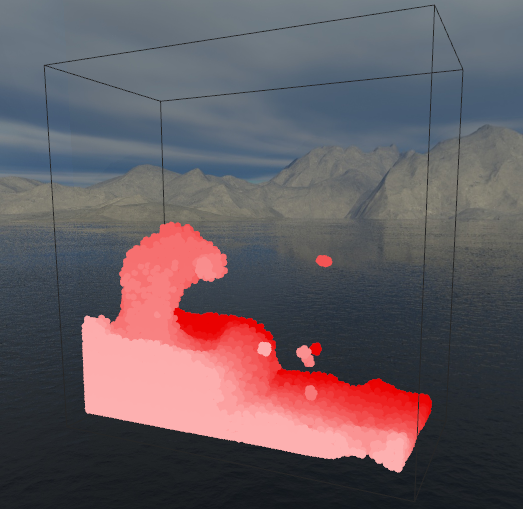
\includegraphics[width=0.7\textwidth]{front_sim}
\caption{Ujęcie z symulacji 16000 cząsteczek. Kolor cząsteczek oznacza numer indeksu oczka siatki do której należą i jednocześnie rozmieszczenie w pamięci}
\label{fig:ss_front_sim}
\end{figure}

\par

\subsection{Prezentacja symulacji}
 
\paragraph{}
\begin{figure}[H]
\centering     %%% not \center

\begin{subfigure}[b]{0.3\textwidth}
\includegraphics[width=\textwidth]{8k/png/image01}%width=0.9\linewidth, keepaspectratio
\end{subfigure}
~
\begin{subfigure}[b]{0.3\textwidth}
\includegraphics[width=\textwidth]{8k/png/image02}%width=0.9\linewidth, keepaspectratio
\end{subfigure}
~
\begin{subfigure}[b]{0.3\textwidth}
\includegraphics[width=\textwidth]{8k/png/image03}%width=0.9\linewidth, keepaspectratio
\end{subfigure}
\\
\vspace{1em}
\begin{subfigure}[b]{0.3\textwidth}
\includegraphics[width=\textwidth]{8k/png/image04}%width=0.9\linewidth, keepaspectratio
\end{subfigure}
~
\begin{subfigure}[b]{0.3\textwidth}
\includegraphics[width=\textwidth]{8k/png/image05}%width=0.9\linewidth, keepaspectratio
\end{subfigure}
~
\begin{subfigure}[b]{0.3\textwidth}
\includegraphics[width=\textwidth]{8k/png/image06}%width=0.9\linewidth, keepaspectratio
\end{subfigure}
\\
\vspace{1em}
\begin{subfigure}[b]{0.3\textwidth}
\includegraphics[width=\textwidth]{8k/png/image07}%width=0.9\linewidth, keepaspectratio
\end{subfigure}
~
\begin{subfigure}[b]{0.3\textwidth}
\includegraphics[width=\textwidth]{8k/png/image08}%width=0.9\linewidth, keepaspectratio
\end{subfigure}
~
\begin{subfigure}[b]{0.3\textwidth}
\includegraphics[width=\textwidth]{8k/png/image09}%width=0.9\linewidth, keepaspectratio
\end{subfigure}

\caption{Ujęcia symulacji w odstępach czasowych około 0.3}
\label{fig:ss_8k}
\end{figure}

\par
Seria ujęć \eqref{fig:ss_8k} przedstawia przykładowy przebieg symulacji płynu. Kolor cząsteczek zależy od ich położenia na siatce wyszukiwania sąsiadów, a jednocześnie świadczą o ułożeniu w pamięci.

\begin{figure}[H]
\centering     %%% not \center

\begin{subfigure}[b]{0.3\textwidth}
\includegraphics[width=\textwidth]{8k_vis_64/image01}%width=0.9\linewidth, keepaspectratio
\end{subfigure}
~
\begin{subfigure}[b]{0.3\textwidth}
\includegraphics[width=\textwidth]{8k_vis_64/image02}%width=0.9\linewidth, keepaspectratio
\end{subfigure}
~
\begin{subfigure}[b]{0.3\textwidth}
\includegraphics[width=\textwidth]{8k_vis_64/image03}%width=0.9\linewidth, keepaspectratio
\end{subfigure}
\\
\vspace{1em}
\begin{subfigure}[b]{0.3\textwidth}
\includegraphics[width=\textwidth]{8k_vis_64/image04}%width=0.9\linewidth, keepaspectratio
\end{subfigure}
~
\begin{subfigure}[b]{0.3\textwidth}
\includegraphics[width=\textwidth]{8k_vis_64/image05}%width=0.9\linewidth, keepaspectratio
\end{subfigure}
~
\begin{subfigure}[b]{0.3\textwidth}
\includegraphics[width=\textwidth]{8k_vis_64/image06}%width=0.9\linewidth, keepaspectratio
\end{subfigure}
\\
\vspace{1em}
\begin{subfigure}[b]{0.3\textwidth}
\includegraphics[width=\textwidth]{8k_vis_64/image07}%width=0.9\linewidth, keepaspectratio
\end{subfigure}
~
\begin{subfigure}[b]{0.3\textwidth}
\includegraphics[width=\textwidth]{8k_vis_64/image08}%width=0.9\linewidth, keepaspectratio
\end{subfigure}
~
\begin{subfigure}[b]{0.3\textwidth}
\includegraphics[width=\textwidth]{8k_vis_64/image09}%width=0.9\linewidth, keepaspectratio
\end{subfigure}

\caption{Ujęcia wizualizacji symulacji w odstępach czasowych równych około 0.3. Siatka wokseli jest rozdzielczości $64^3$}
\label{fig:ss_8k_vis_64}
\end{figure}

\par
Seria ujęć \eqref{fig:ss_8k_vis_64} odpowiada wizualizacji przebiegu symulacji pokazanej na \eqref{fig:ss_8k}, przy wykorzystaniu siatki wokseli o rozdzielczości $64^3$. Na ujęciach została wykorzystana technika mapowanie kubicznego (ang. cube mapping), która ma za zadanie symulować załamania promieni światła przechodzących przez objętość płynu.

\begin{figure}[H]
\centering     %%% not \center

\begin{subfigure}[b]{0.80\textwidth}
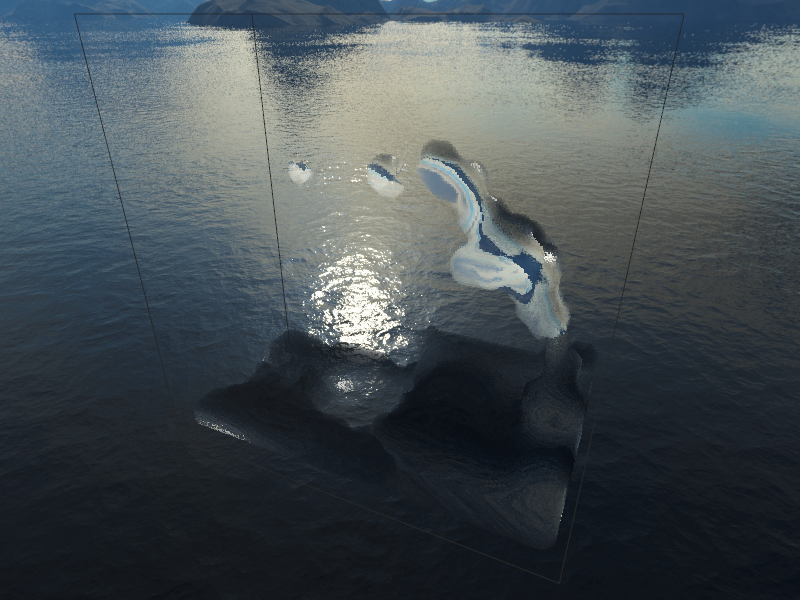
\includegraphics[width=\textwidth]{8k_vis_comp/image32}%width=0.9\linewidth, keepaspectratio
\caption{Rozdzielczość siatki wokseli: $32\cross32\cross32$}
\label{subfig:ss_8k_comp_32}
\end{subfigure}
%~
\\
\vspace{1em}
\begin{subfigure}[b]{0.80\textwidth}
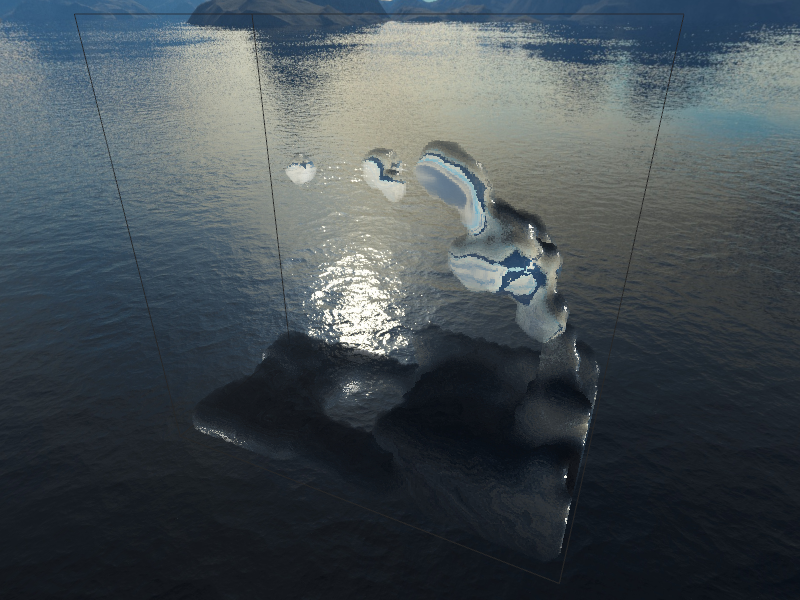
\includegraphics[width=\textwidth]{8k_vis_comp/image64}%width=0.9\linewidth, keepaspectratio
\caption{Rozdzielczość siatki wokseli: $64\cross64\cross64$}
\label{subfig:ss_8k_comp_64}
\end{subfigure}

\caption{Porównanie jakości wizualizacji dla różnych rozdzielczości siatek wokseli: $32^3$ i $64^3$}
\label{fig:ss_8k_comp_32_64}
\end{figure}

\par
Ujęcia \eqref{fig:ss_8k_comp_32_64} przedstawiają tę samą chwilę czasową. Wizualizacja została przeprowadzona jednak z różną dokładnością próbkowania płynu na mapie odległości. Ujęcie \eqref{subfig:ss_8k_comp_64} prezentuje więcej szczegółów, załamania promieni przez powierzchnię płynu wydają się być bardziej naturalne (spowodowane jest to zwiększoną dokładnością obliczenia wektorów normalnych powierzchni).
\par

\begin{figure}[H]
\centering     %%% not \center

\begin{subfigure}[b]{0.45\textwidth}
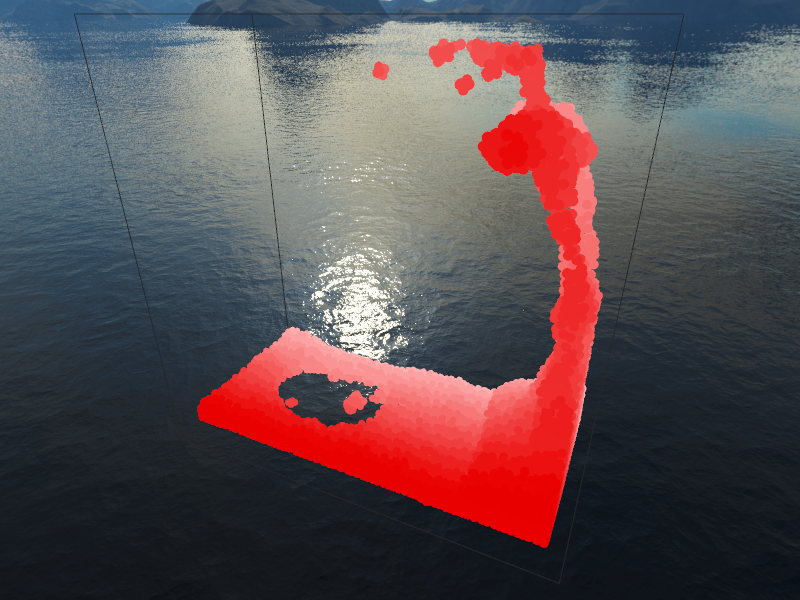
\includegraphics[width=\textwidth]{8k_viscosity_comp/viscosity01}
\caption{Stała lepkości $\mu=1.5$}
\label{subfig:ss_8k_comp_viscosity_15_1}
\end{subfigure}
~
\begin{subfigure}[b]{0.45\textwidth}
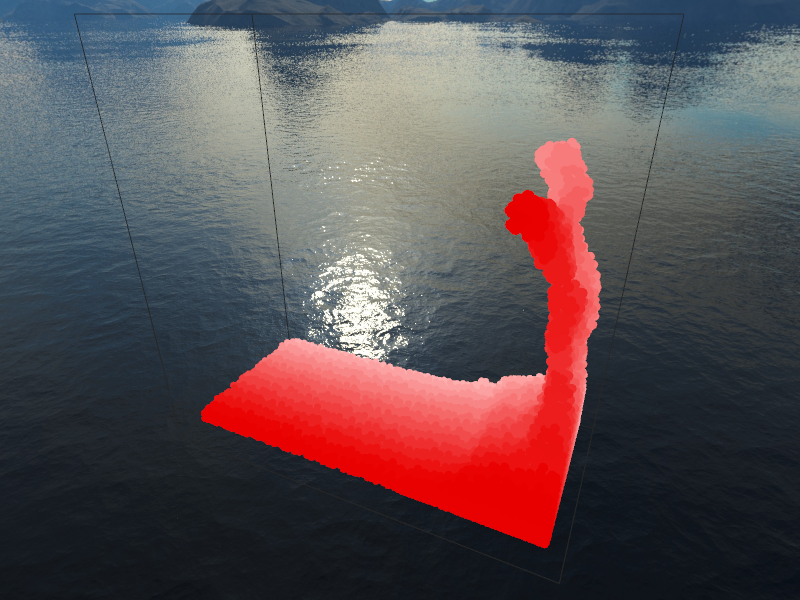
\includegraphics[width=\textwidth]{8k_viscosity_comp/viscosity01_5}
\caption{Stała lepkości $\mu=5.0$}
\label{subfig:ss_8k_comp_viscosity_50_1}
\end{subfigure}
\\
\vspace{1em}
\begin{subfigure}[b]{0.45\textwidth}
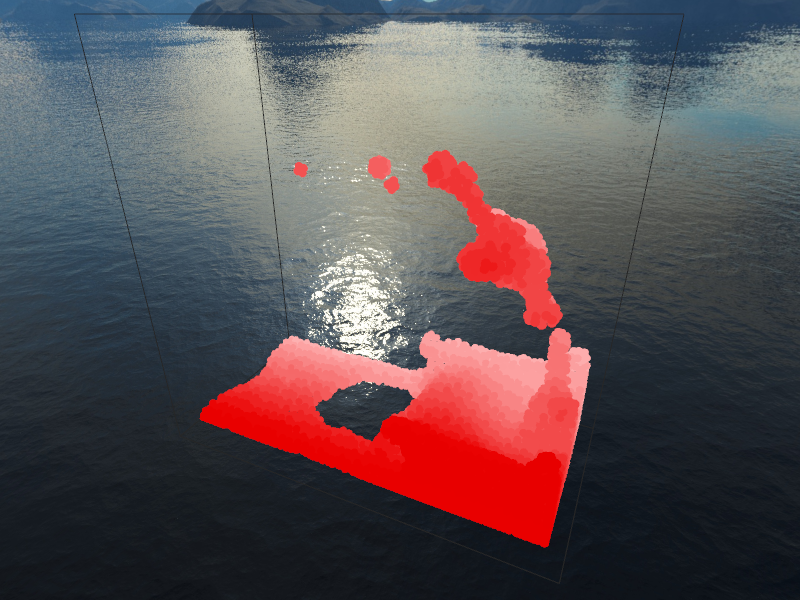
\includegraphics[width=\textwidth]{8k_viscosity_comp/viscosity02}
\caption{Stała lepkości $\mu=1.5$}
\label{subfig:ss_8k_comp_viscosity_15_2}
\end{subfigure}
~
\begin{subfigure}[b]{0.45\textwidth}
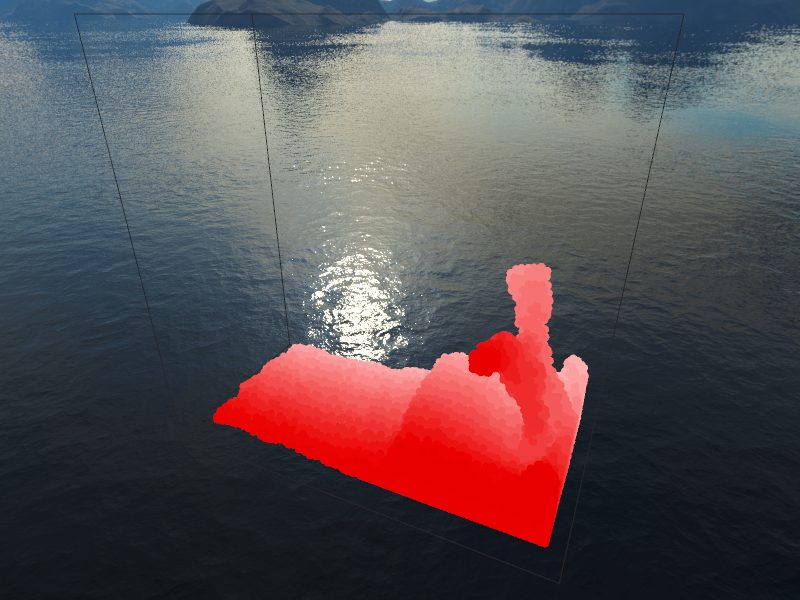
\includegraphics[width=\textwidth]{8k_viscosity_comp/viscosity02_5}
\caption{Stała lepkości $\mu=5.0$}
\label{subfig:ss_8k_comp_viscosity_50_2}
\end{subfigure}

\caption{Porównanie przebiegu symulacji dla róznych wartości stałej lepkości $\mu$: $1.5$ i $5.0$}
\label{fig:ss_8k_comp_viscosity}
\end{figure}

\par
Ujęcia \eqref{fig:ss_8k_comp_viscosity} pokazują wizualne różnice w symulacji przy różnych wartościach stałej lepkości. Można zauważyć, że zachowanie płynu przy mniejszej lepkości jest bardziej gwałtowne, burzliwe. Dla płynu o większej lepkości prędkość cząsteczek jest tracona przez wewnętrzne tarcie. Ten efekt dodatkowo można zaobserwować na wykresie \eqref{fig:plot_viscosity}.

\subsection{Analiza wydajności}
\label{subsec:perf_anal}

\paragraph{}
Poniżej przedstawione zostały wyniki wydajności stworzonej aplikacji. Celem tego akapitu, oprócz podbudowania ego autora wysokimi słupkami wydajności widocznymi na wykresach, jest wskazanie progu ilości cząsteczek aby symulację wciąż można było uznać za interaktywną (czyli taką, w której ze swobodą można manipulować aplikacją w czasie rzeczywistym). Z drugiej strony, granicą płynności animacji (która jest subiektywna i przedstawiona tutaj wartość wynika z własnych doświadczeń autora z aplikacją) jest około 12-15 klatkek na sekundę.
\par

\begin{figure}[H]
% GNUPLOT: LaTeX picture with Postscript
\begingroup
  \fontshape{sc}%
  \selectfont
\bfseries
\fontsize{10}{12}
\selectfont
  \makeatletter
  \providecommand\color[2][]{%
    \GenericError{(gnuplot) \space\space\space\@spaces}{%
      Package color not loaded in conjunction with
      terminal option `colourtext'%
    }{See the gnuplot documentation for explanation.%
    }{Either use 'blacktext' in gnuplot or load the package
      color.sty in LaTeX.}%
    \renewcommand\color[2][]{}%
  }%
  \providecommand\includegraphics[2][]{%
    \GenericError{(gnuplot) \space\space\space\@spaces}{%
      Package graphicx or graphics not loaded%
    }{See the gnuplot documentation for explanation.%
    }{The gnuplot epslatex terminal needs graphicx.sty or graphics.sty.}%
    \renewcommand\includegraphics[2][]{}%
  }%
  \providecommand\rotatebox[2]{#2}%
  \@ifundefined{ifGPcolor}{%
    \newif\ifGPcolor
    \GPcolortrue
  }{}%
  \@ifundefined{ifGPblacktext}{%
    \newif\ifGPblacktext
    \GPblacktextfalse
  }{}%
  % define a \g@addto@macro without @ in the name:
  \let\gplgaddtomacro\g@addto@macro
  % define empty templates for all commands taking text:
  \gdef\gplbacktext{}%
  \gdef\gplfronttext{}%
  \makeatother
  \ifGPblacktext
    % no textcolor at all
    \def\colorrgb#1{}%
    \def\colorgray#1{}%
  \else
    % gray or color?
    \ifGPcolor
      \def\colorrgb#1{\color[rgb]{#1}}%
      \def\colorgray#1{\color[gray]{#1}}%
      \expandafter\def\csname LTw\endcsname{\color{white}}%
      \expandafter\def\csname LTb\endcsname{\color{black}}%
      \expandafter\def\csname LTa\endcsname{\color{black}}%
      \expandafter\def\csname LT0\endcsname{\color[rgb]{1,0,0}}%
      \expandafter\def\csname LT1\endcsname{\color[rgb]{0,1,0}}%
      \expandafter\def\csname LT2\endcsname{\color[rgb]{0,0,1}}%
      \expandafter\def\csname LT3\endcsname{\color[rgb]{1,0,1}}%
      \expandafter\def\csname LT4\endcsname{\color[rgb]{0,1,1}}%
      \expandafter\def\csname LT5\endcsname{\color[rgb]{1,1,0}}%
      \expandafter\def\csname LT6\endcsname{\color[rgb]{0,0,0}}%
      \expandafter\def\csname LT7\endcsname{\color[rgb]{1,0.3,0}}%
      \expandafter\def\csname LT8\endcsname{\color[rgb]{0.5,0.5,0.5}}%
    \else
      % gray
      \def\colorrgb#1{\color{black}}%
      \def\colorgray#1{\color[gray]{#1}}%
      \expandafter\def\csname LTw\endcsname{\color{white}}%
      \expandafter\def\csname LTb\endcsname{\color{black}}%
      \expandafter\def\csname LTa\endcsname{\color{black}}%
      \expandafter\def\csname LT0\endcsname{\color{black}}%
      \expandafter\def\csname LT1\endcsname{\color{black}}%
      \expandafter\def\csname LT2\endcsname{\color{black}}%
      \expandafter\def\csname LT3\endcsname{\color{black}}%
      \expandafter\def\csname LT4\endcsname{\color{black}}%
      \expandafter\def\csname LT5\endcsname{\color{black}}%
      \expandafter\def\csname LT6\endcsname{\color{black}}%
      \expandafter\def\csname LT7\endcsname{\color{black}}%
      \expandafter\def\csname LT8\endcsname{\color{black}}%
    \fi
  \fi
    \setlength{\unitlength}{0.0500bp}%
    \ifx\gptboxheight\undefined%
      \newlength{\gptboxheight}%
      \newlength{\gptboxwidth}%
      \newsavebox{\gptboxtext}%
    \fi%
    \setlength{\fboxrule}{0.5pt}%
    \setlength{\fboxsep}{1pt}%
\begin{picture}(9920.00,6802.00)%
    \gplgaddtomacro\gplbacktext{%
      \csname LTb\endcsname%
      \put(682,704){\makebox(0,0)[r]{\strut{}$\mathtt{0}$}}%
      \put(682,1472){\makebox(0,0)[r]{\strut{}$\mathtt{10}$}}%
      \put(682,2239){\makebox(0,0)[r]{\strut{}$\mathtt{20}$}}%
      \put(682,3007){\makebox(0,0)[r]{\strut{}$\mathtt{30}$}}%
      \put(682,3774){\makebox(0,0)[r]{\strut{}$\mathtt{40}$}}%
      \put(682,4542){\makebox(0,0)[r]{\strut{}$\mathtt{50}$}}%
      \put(682,5309){\makebox(0,0)[r]{\strut{}$\mathtt{60}$}}%
      \put(682,6077){\makebox(0,0)[r]{\strut{}$\mathtt{70}$}}%
      \put(1436,484){\makebox(0,0){\strut{}$\mathtt{1\times1\times1}$}}%
      \put(2680,484){\makebox(0,0){\strut{}$\mathtt{2\times2\times1}$}}%
      \put(3924,484){\makebox(0,0){\strut{}$\mathtt{4\times4\times2}$}}%
      \put(5169,484){\makebox(0,0){\strut{}$\mathtt{8\times8\times4}$}}%
      \put(6413,484){\makebox(0,0){\strut{}$\mathtt{16\times16\times8}$}}%
      \put(7657,484){\makebox(0,0){\strut{}$\mathtt{32\times32\times16}$}}%
      \put(8901,484){\makebox(0,0){\strut{}$\mathtt{64\times64\times32}$}}%
    }%
    \gplgaddtomacro\gplfronttext{%
      \csname LTb\endcsname%
      \put(176,3620){\rotatebox{-270}{\makebox(0,0){\strut{}klatki na sekundę}}}%
      \put(5168,154){\makebox(0,0){\strut{}rozdzielczość siatki sąsiadów $\mathtt{K \times L \times M}$}}%
      \csname LTb\endcsname%
      \put(8536,6364){\makebox(0,0)[r]{\strut{}max}}%
      \csname LTb\endcsname%
      \put(1436,1433){\makebox(0,0){\strut{}8}}%
      \put(2680,1433){\makebox(0,0){\strut{}8}}%
      \put(3924,1663){\makebox(0,0){\strut{}11}}%
      \put(5169,2508){\makebox(0,0){\strut{}22}}%
      \put(6413,3812){\makebox(0,0){\strut{}39}}%
      \put(7657,4810){\makebox(0,0){\strut{}52}}%
      \put(8901,5578){\makebox(0,0){\strut{}62}}%
      \csname LTb\endcsname%
      \put(8536,6144){\makebox(0,0)[r]{\strut{}avg}}%
      \csname LTb\endcsname%
      \put(1996,1263){\makebox(0,0){\strut{}7.28}}%
      \put(3240,1257){\makebox(0,0){\strut{}7.21}}%
      \put(4484,1397){\makebox(0,0){\strut{}9.03}}%
      \put(5728,2085){\makebox(0,0){\strut{}17.99}}%
      \put(6973,3265){\makebox(0,0){\strut{}33.37}}%
      \put(8217,4376){\makebox(0,0){\strut{}47.84}}%
      \put(9461,5309){\makebox(0,0){\strut{}60.00}}%
      \csname LTb\endcsname%
      \put(8536,5924){\makebox(0,0)[r]{\strut{}min}}%
      \csname LTb\endcsname%
      \put(1436,1088){\makebox(0,0){\strut{}7}}%
      \put(2680,1011){\makebox(0,0){\strut{}6}}%
      \put(3924,1088){\makebox(0,0){\strut{}7}}%
      \put(5169,1318){\makebox(0,0){\strut{}10}}%
      \put(6413,2393){\makebox(0,0){\strut{}24}}%
      \put(7657,3697){\makebox(0,0){\strut{}41}}%
      \put(8901,5079){\makebox(0,0){\strut{}59}}%
    }%
    \gplbacktext
    \put(0,0){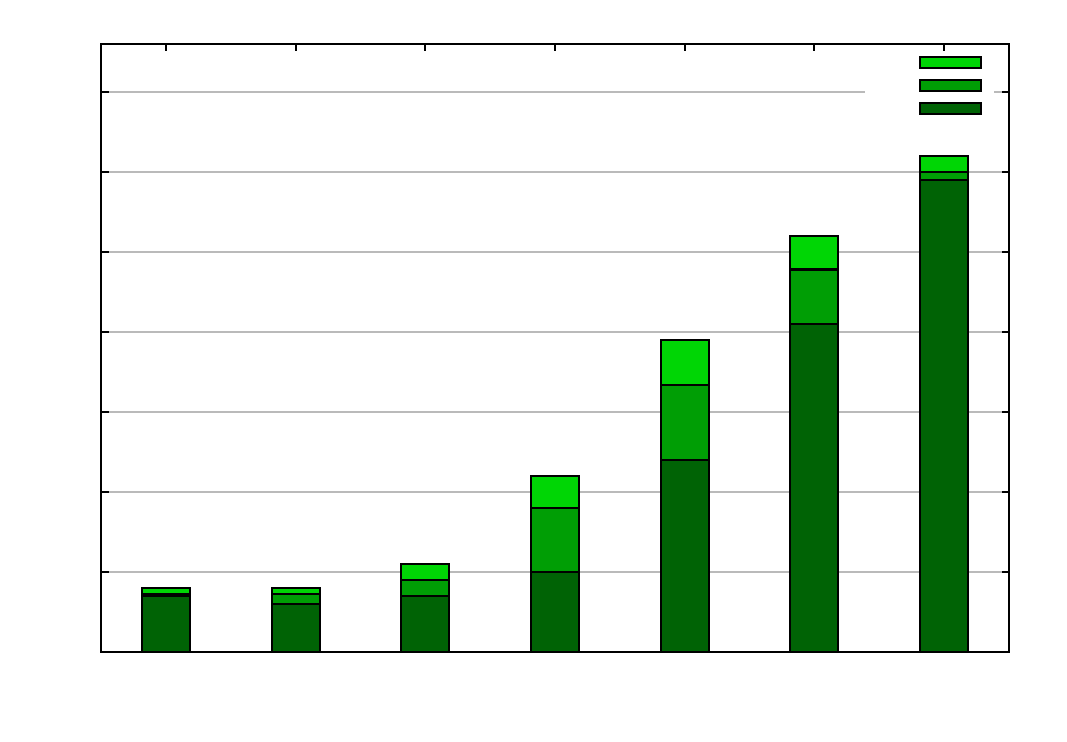
\includegraphics{fps_grid_res}}%
    \gplfronttext
  \end{picture}%
\endgroup

\caption{Wykres wydajności wyrażonej w klatkach na sekundę w zależności od rozdzielczości siatki przeszukiwania sąsiadów. Przedstawione wartości są wynikiem symulowania $2000$ cząsteczek. Uwaga - ostatni słupek pokazuje przekłamane wartości (wyjaśnienie poniżej)}
\label{fig:plot_grid_resolution_perf}
\end{figure}

\par
Wykres \eqref{fig:plot_grid_resolution_perf} obrazuje skuteczność zaproponowanego algorytmu wyszukiwania sąsiadów. Wydajność zoptymalizowanej symulacji (przedostatni słupek $32\cross32\cross16$) w porównaniu do symulacji bez optymalizacji (pierwszy słupek $1\cross1\cross1$) wzrosta około 5-krotnie.
\par
Trzeba zaznaczyć, że przyrost wydajności na ostatnim słupku nie jest w pełni prawdziwy. Wynika to z dwóch rzeczy.
\par
Przy przeprowadzaniu testów ustawienia sterowników karty graficznej wymuszały tzw. synchronizację pionową. Funkcja ta ma wyeliminować błędy wyświetlania obrazu charakterystyczne dla monitorów LCD (przede wszystkim tzw. rozrywanie obrazu [ang. screen tearing]). Włączenie tego mechanizmu powoduje jednak ogranicznie liczby wyświetlanych klatek do częstotliwości odświeżania monitora, która w wypadku konfiguracji testowej wynosiła 60 Hz.
\par
Drugim powodem przekłamania na wykresie jest zbyt duża rozdzielczość siatki. W tym ostatnim przypadku pojedyncze oczko siatki ma rozmiary mniejsze niż promień jądra wygładzającego i z tego powodu cząsteczki nie znajdują wszystkich swoich sąsiadów. W rezultacie siły są błędnie obliczane i zachowanie płynu odbiega od spodziewanego.

\begin{figure}[H]
% GNUPLOT: LaTeX picture with Postscript
\begingroup
  \fontshape{sc}%
  \selectfont
\bfseries
\fontsize{10}{12}
\selectfont
  \makeatletter
  \providecommand\color[2][]{%
    \GenericError{(gnuplot) \space\space\space\@spaces}{%
      Package color not loaded in conjunction with
      terminal option `colourtext'%
    }{See the gnuplot documentation for explanation.%
    }{Either use 'blacktext' in gnuplot or load the package
      color.sty in LaTeX.}%
    \renewcommand\color[2][]{}%
  }%
  \providecommand\includegraphics[2][]{%
    \GenericError{(gnuplot) \space\space\space\@spaces}{%
      Package graphicx or graphics not loaded%
    }{See the gnuplot documentation for explanation.%
    }{The gnuplot epslatex terminal needs graphicx.sty or graphics.sty.}%
    \renewcommand\includegraphics[2][]{}%
  }%
  \providecommand\rotatebox[2]{#2}%
  \@ifundefined{ifGPcolor}{%
    \newif\ifGPcolor
    \GPcolortrue
  }{}%
  \@ifundefined{ifGPblacktext}{%
    \newif\ifGPblacktext
    \GPblacktextfalse
  }{}%
  % define a \g@addto@macro without @ in the name:
  \let\gplgaddtomacro\g@addto@macro
  % define empty templates for all commands taking text:
  \gdef\gplbacktext{}%
  \gdef\gplfronttext{}%
  \makeatother
  \ifGPblacktext
    % no textcolor at all
    \def\colorrgb#1{}%
    \def\colorgray#1{}%
  \else
    % gray or color?
    \ifGPcolor
      \def\colorrgb#1{\color[rgb]{#1}}%
      \def\colorgray#1{\color[gray]{#1}}%
      \expandafter\def\csname LTw\endcsname{\color{white}}%
      \expandafter\def\csname LTb\endcsname{\color{black}}%
      \expandafter\def\csname LTa\endcsname{\color{black}}%
      \expandafter\def\csname LT0\endcsname{\color[rgb]{1,0,0}}%
      \expandafter\def\csname LT1\endcsname{\color[rgb]{0,1,0}}%
      \expandafter\def\csname LT2\endcsname{\color[rgb]{0,0,1}}%
      \expandafter\def\csname LT3\endcsname{\color[rgb]{1,0,1}}%
      \expandafter\def\csname LT4\endcsname{\color[rgb]{0,1,1}}%
      \expandafter\def\csname LT5\endcsname{\color[rgb]{1,1,0}}%
      \expandafter\def\csname LT6\endcsname{\color[rgb]{0,0,0}}%
      \expandafter\def\csname LT7\endcsname{\color[rgb]{1,0.3,0}}%
      \expandafter\def\csname LT8\endcsname{\color[rgb]{0.5,0.5,0.5}}%
    \else
      % gray
      \def\colorrgb#1{\color{black}}%
      \def\colorgray#1{\color[gray]{#1}}%
      \expandafter\def\csname LTw\endcsname{\color{white}}%
      \expandafter\def\csname LTb\endcsname{\color{black}}%
      \expandafter\def\csname LTa\endcsname{\color{black}}%
      \expandafter\def\csname LT0\endcsname{\color{black}}%
      \expandafter\def\csname LT1\endcsname{\color{black}}%
      \expandafter\def\csname LT2\endcsname{\color{black}}%
      \expandafter\def\csname LT3\endcsname{\color{black}}%
      \expandafter\def\csname LT4\endcsname{\color{black}}%
      \expandafter\def\csname LT5\endcsname{\color{black}}%
      \expandafter\def\csname LT6\endcsname{\color{black}}%
      \expandafter\def\csname LT7\endcsname{\color{black}}%
      \expandafter\def\csname LT8\endcsname{\color{black}}%
    \fi
  \fi
    \setlength{\unitlength}{0.0500bp}%
    \ifx\gptboxheight\undefined%
      \newlength{\gptboxheight}%
      \newlength{\gptboxwidth}%
      \newsavebox{\gptboxtext}%
    \fi%
    \setlength{\fboxrule}{0.5pt}%
    \setlength{\fboxsep}{1pt}%
\begin{picture}(9920.00,6802.00)%
    \gplgaddtomacro\gplbacktext{%
      \csname LTb\endcsname%
      \put(682,704){\makebox(0,0)[r]{\strut{}$0$}}%
      \csname LTb\endcsname%
      \put(682,1676){\makebox(0,0)[r]{\strut{}$10$}}%
      \csname LTb\endcsname%
      \put(682,2648){\makebox(0,0)[r]{\strut{}$20$}}%
      \csname LTb\endcsname%
      \put(682,3621){\makebox(0,0)[r]{\strut{}$30$}}%
      \csname LTb\endcsname%
      \put(682,4593){\makebox(0,0)[r]{\strut{}$40$}}%
      \csname LTb\endcsname%
      \put(682,5565){\makebox(0,0)[r]{\strut{}$50$}}%
      \csname LTb\endcsname%
      \put(682,6537){\makebox(0,0)[r]{\strut{}$60$}}%
      \put(1436,484){\makebox(0,0){\strut{}$\mathtt{2000}$}}%
      \put(2680,484){\makebox(0,0){\strut{}$\mathtt{3000}$}}%
      \put(3924,484){\makebox(0,0){\strut{}$\mathtt{4000}$}}%
      \put(5169,484){\makebox(0,0){\strut{}$\mathtt{6000}$}}%
      \put(6413,484){\makebox(0,0){\strut{}$\mathtt{8000}$}}%
      \put(7657,484){\makebox(0,0){\strut{}$\mathtt{12000}$}}%
      \put(8901,484){\makebox(0,0){\strut{}$\mathtt{16000}$}}%
    }%
    \gplgaddtomacro\gplfronttext{%
      \csname LTb\endcsname%
      \put(176,3620){\rotatebox{-270}{\makebox(0,0){\strut{}klatki na sekundę}}}%
      \put(5168,154){\makebox(0,0){\strut{}liczba cząsteczek $\mathtt{n}$}}%
      \csname LTb\endcsname%
      \put(8536,6364){\makebox(0,0)[r]{\strut{}max}}%
      \csname LTb\endcsname%
      \put(1436,5905){\makebox(0,0){\strut{}52}}%
      \put(2680,3961){\makebox(0,0){\strut{}32}}%
      \put(3924,3086){\makebox(0,0){\strut{}23}}%
      \put(5169,2308){\makebox(0,0){\strut{}15}}%
      \put(6413,1919){\makebox(0,0){\strut{}11}}%
      \put(7657,1530){\makebox(0,0){\strut{}7}}%
      \put(8901,1336){\makebox(0,0){\strut{}5}}%
      \csname LTb\endcsname%
      \put(8536,6144){\makebox(0,0)[r]{\strut{}avg}}%
      \csname LTb\endcsname%
      \put(1996,5355){\makebox(0,0){\strut{}47.84}}%
      \put(3240,3569){\makebox(0,0){\strut{}29.47}}%
      \put(4484,2751){\makebox(0,0){\strut{}21.06}}%
      \put(5728,1955){\makebox(0,0){\strut{}12.87}}%
      \put(6973,1600){\makebox(0,0){\strut{}9.22}}%
      \put(8217,1252){\makebox(0,0){\strut{}5.64}}%
      \put(9461,1094){\makebox(0,0){\strut{}4.01}}%
      \csname LTb\endcsname%
      \put(8536,5924){\makebox(0,0)[r]{\strut{}min}}%
      \csname LTb\endcsname%
      \put(1436,4495){\makebox(0,0){\strut{}41}}%
      \put(2680,2940){\makebox(0,0){\strut{}25}}%
      \put(3924,2162){\makebox(0,0){\strut{}17}}%
      \put(5169,1482){\makebox(0,0){\strut{}10}}%
      \put(6413,1190){\makebox(0,0){\strut{}7}}%
      \put(7657,898){\makebox(0,0){\strut{}4}}%
      \put(8901,801){\makebox(0,0){\strut{}3}}%
    }%
    \gplbacktext
    \put(0,0){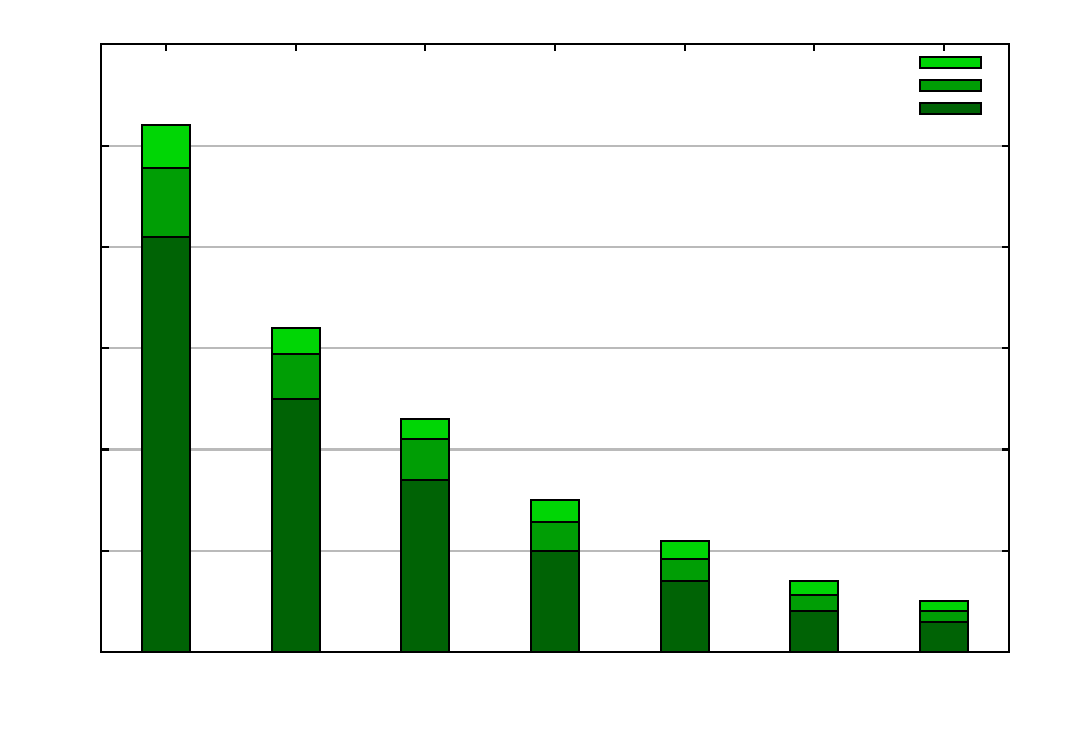
\includegraphics{fps_n}}%
    \gplfronttext
  \end{picture}%
\endgroup

\caption{Wykres wydajności wyrażonej w klatkach na sekundę w zależności od liczby cząsteczek biorących udział w symulacji}
\label{fig:plot_particles_perf}
\end{figure}

\par
Wykres \eqref{fig:plot_particles_perf} obrazuje wpływ ilości symulowanych cząsteczek na wydajność. Na jego podstawie można ocenić, że interaktywność symulacji zachowana jest dla ok. $6000$ cząsteczek.

\begin{figure}[H]
\centering
% GNUPLOT: LaTeX picture with Postscript
\begingroup
  \fontshape{sc}%
  \selectfont
\bfseries
\fontsize{10}{12}
\selectfont
  \makeatletter
  \providecommand\color[2][]{%
    \GenericError{(gnuplot) \space\space\space\@spaces}{%
      Package color not loaded in conjunction with
      terminal option `colourtext'%
    }{See the gnuplot documentation for explanation.%
    }{Either use 'blacktext' in gnuplot or load the package
      color.sty in LaTeX.}%
    \renewcommand\color[2][]{}%
  }%
  \providecommand\includegraphics[2][]{%
    \GenericError{(gnuplot) \space\space\space\@spaces}{%
      Package graphicx or graphics not loaded%
    }{See the gnuplot documentation for explanation.%
    }{The gnuplot epslatex terminal needs graphicx.sty or graphics.sty.}%
    \renewcommand\includegraphics[2][]{}%
  }%
  \providecommand\rotatebox[2]{#2}%
  \@ifundefined{ifGPcolor}{%
    \newif\ifGPcolor
    \GPcolortrue
  }{}%
  \@ifundefined{ifGPblacktext}{%
    \newif\ifGPblacktext
    \GPblacktextfalse
  }{}%
  % define a \g@addto@macro without @ in the name:
  \let\gplgaddtomacro\g@addto@macro
  % define empty templates for all commands taking text:
  \gdef\gplbacktext{}%
  \gdef\gplfronttext{}%
  \makeatother
  \ifGPblacktext
    % no textcolor at all
    \def\colorrgb#1{}%
    \def\colorgray#1{}%
  \else
    % gray or color?
    \ifGPcolor
      \def\colorrgb#1{\color[rgb]{#1}}%
      \def\colorgray#1{\color[gray]{#1}}%
      \expandafter\def\csname LTw\endcsname{\color{white}}%
      \expandafter\def\csname LTb\endcsname{\color{black}}%
      \expandafter\def\csname LTa\endcsname{\color{black}}%
      \expandafter\def\csname LT0\endcsname{\color[rgb]{1,0,0}}%
      \expandafter\def\csname LT1\endcsname{\color[rgb]{0,1,0}}%
      \expandafter\def\csname LT2\endcsname{\color[rgb]{0,0,1}}%
      \expandafter\def\csname LT3\endcsname{\color[rgb]{1,0,1}}%
      \expandafter\def\csname LT4\endcsname{\color[rgb]{0,1,1}}%
      \expandafter\def\csname LT5\endcsname{\color[rgb]{1,1,0}}%
      \expandafter\def\csname LT6\endcsname{\color[rgb]{0,0,0}}%
      \expandafter\def\csname LT7\endcsname{\color[rgb]{1,0.3,0}}%
      \expandafter\def\csname LT8\endcsname{\color[rgb]{0.5,0.5,0.5}}%
    \else
      % gray
      \def\colorrgb#1{\color{black}}%
      \def\colorgray#1{\color[gray]{#1}}%
      \expandafter\def\csname LTw\endcsname{\color{white}}%
      \expandafter\def\csname LTb\endcsname{\color{black}}%
      \expandafter\def\csname LTa\endcsname{\color{black}}%
      \expandafter\def\csname LT0\endcsname{\color{black}}%
      \expandafter\def\csname LT1\endcsname{\color{black}}%
      \expandafter\def\csname LT2\endcsname{\color{black}}%
      \expandafter\def\csname LT3\endcsname{\color{black}}%
      \expandafter\def\csname LT4\endcsname{\color{black}}%
      \expandafter\def\csname LT5\endcsname{\color{black}}%
      \expandafter\def\csname LT6\endcsname{\color{black}}%
      \expandafter\def\csname LT7\endcsname{\color{black}}%
      \expandafter\def\csname LT8\endcsname{\color{black}}%
    \fi
  \fi
    \setlength{\unitlength}{0.0500bp}%
    \ifx\gptboxheight\undefined%
      \newlength{\gptboxheight}%
      \newlength{\gptboxwidth}%
      \newsavebox{\gptboxtext}%
    \fi%
    \setlength{\fboxrule}{0.5pt}%
    \setlength{\fboxsep}{1pt}%
\begin{picture}(8786.00,5668.00)%
    \gplgaddtomacro\gplbacktext{%
      \csname LTb\endcsname%
      \put(682,704){\makebox(0,0)[r]{\strut{}$0$}}%
      \csname LTb\endcsname%
      \put(682,1644){\makebox(0,0)[r]{\strut{}$5$}}%
      \csname LTb\endcsname%
      \put(682,2584){\makebox(0,0)[r]{\strut{}$10$}}%
      \csname LTb\endcsname%
      \put(682,3523){\makebox(0,0)[r]{\strut{}$15$}}%
      \csname LTb\endcsname%
      \put(682,4463){\makebox(0,0)[r]{\strut{}$20$}}%
      \csname LTb\endcsname%
      \put(682,5403){\makebox(0,0)[r]{\strut{}$25$}}%
      \put(3070,484){\makebox(0,0){\strut{}$\mathtt{2000}$}}%
      \put(6294,484){\makebox(0,0){\strut{}$\mathtt{4000}$}}%
    }%
    \gplgaddtomacro\gplfronttext{%
      \csname LTb\endcsname%
      \put(176,3053){\rotatebox{-270}{\makebox(0,0){\strut{}klatki na sekundę}}}%
      \put(4601,154){\makebox(0,0){\strut{}liczba cząsteczek $\mathtt{n}$}}%
      \csname LTb\endcsname%
      \put(7402,5230){\makebox(0,0)[r]{\strut{}$\mathtt{32^3}$--------}}%
      \csname LTb\endcsname%
      \put(7402,5010){\makebox(0,0)[r]{\strut{}max}}%
      \csname LTb\endcsname%
      \put(2426,4839){\makebox(0,0){\strut{}21}}%
      \put(5649,3147){\makebox(0,0){\strut{}12}}%
      \csname LTb\endcsname%
      \put(7402,4790){\makebox(0,0)[r]{\strut{}avg}}%
      \csname LTb\endcsname%
      \put(1620,4397){\makebox(0,0){\strut{}19.65}}%
      \put(4843,2770){\makebox(0,0){\strut{}10.99}}%
      \csname LTb\endcsname%
      \put(7402,4570){\makebox(0,0)[r]{\strut{}min}}%
      \csname LTb\endcsname%
      \put(2426,3899){\makebox(0,0){\strut{}18}}%
      \put(5649,2208){\makebox(0,0){\strut{}9}}%
      \csname LTb\endcsname%
      \put(7402,4350){\makebox(0,0)[r]{\strut{}$\mathtt{64^3}$--------}}%
      \csname LTb\endcsname%
      \put(7402,4130){\makebox(0,0)[r]{\strut{}max}}%
      \csname LTb\endcsname%
      \put(3554,2020){\makebox(0,0){\strut{}6}}%
      \put(6777,1832){\makebox(0,0){\strut{}5}}%
      \csname LTb\endcsname%
      \put(7402,3910){\makebox(0,0)[r]{\strut{}avg}}%
      \csname LTb\endcsname%
      \put(4360,1815){\makebox(0,0){\strut{}5.91}}%
      \put(7583,1608){\makebox(0,0){\strut{}4.81}}%
      \csname LTb\endcsname%
      \put(7402,3690){\makebox(0,0)[r]{\strut{}min}}%
      \csname LTb\endcsname%
      \put(3554,1456){\makebox(0,0){\strut{}5}}%
      \put(6777,1268){\makebox(0,0){\strut{}4}}%
    }%
    \gplbacktext
    \put(0,0){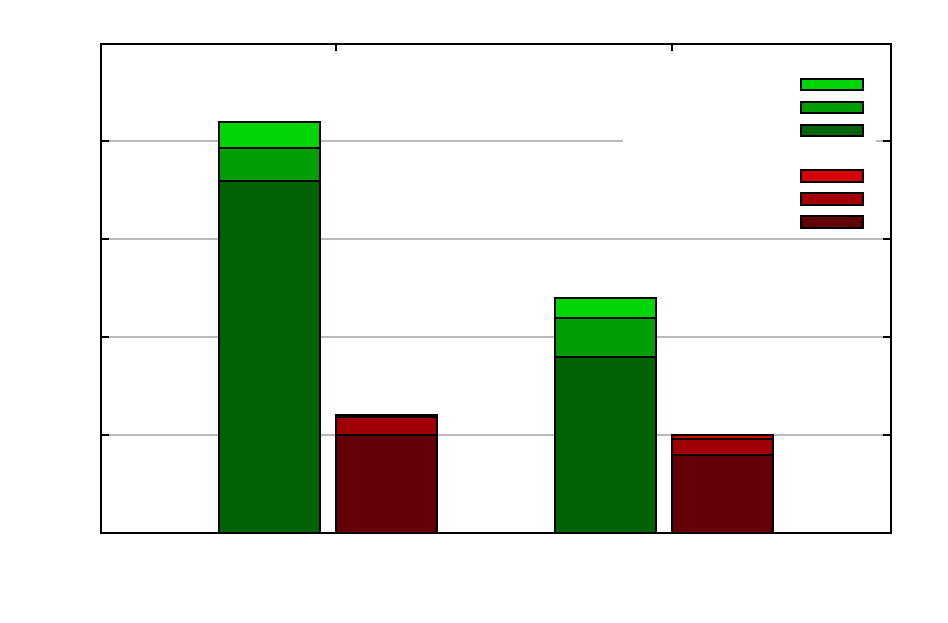
\includegraphics{fps_n_d}}%
    \gplfronttext
  \end{picture}%
\endgroup

\caption{Wykres wydajności symulacji i wizualizacji wyrażonej w klatkach na sekundę w zależności od liczby cząsteczek biorących udział w symulacji oraz od rodzielczości użytej siatki wokseli (siatki $32^3$ i $64^3$)}
\label{fig:plot_particles_vis_perf}
\end{figure}

\par
Wykres \eqref{fig:plot_particles_vis_perf} pokazuje z jaką wydajnością przeprowadzana jest symulacja płynu wraz z jego wizualizacją. W tym wypadku interaktywność symulacji, dla siatki wokseli $32\cross32\cross32$, zachowana jest już dla mniej niż $4000$ cząsteczek. Niestety w przypadku użycia siatki wokseli o większej rozdzielczości ($64^3$) płynność animacji znacząco spada i nawet dla $2000$ cząsteczek nie jest możliwe uzyskanie zadowalającej wydajności.
\par
Porównując ten wykres do wykresu \eqref{fig:plot_particles_perf} można zauważyć, że sam proces wizualizacji jest kosztowny obliczeniowo. Przeniesienie większej ilości obliczeń na kartę graficzną mając na uwadze choćby zmniejszenie transferu danych pomiędzy procesorem a kartą, dałoby prawdopodobnie znaczące przyspieszenie procesu wizualizacji.


\subsection{Analiza stabilności numerycznej}

\paragraph{}
\begin{figure}[H]
% GNUPLOT: LaTeX picture with Postscript
\begingroup
  \makeatletter
  \providecommand\color[2][]{%
    \GenericError{(gnuplot) \space\space\space\@spaces}{%
      Package color not loaded in conjunction with
      terminal option `colourtext'%
    }{See the gnuplot documentation for explanation.%
    }{Either use 'blacktext' in gnuplot or load the package
      color.sty in LaTeX.}%
    \renewcommand\color[2][]{}%
  }%
  \providecommand\includegraphics[2][]{%
    \GenericError{(gnuplot) \space\space\space\@spaces}{%
      Package graphicx or graphics not loaded%
    }{See the gnuplot documentation for explanation.%
    }{The gnuplot epslatex terminal needs graphicx.sty or graphics.sty.}%
    \renewcommand\includegraphics[2][]{}%
  }%
  \providecommand\rotatebox[2]{#2}%
  \@ifundefined{ifGPcolor}{%
    \newif\ifGPcolor
    \GPcolortrue
  }{}%
  \@ifundefined{ifGPblacktext}{%
    \newif\ifGPblacktext
    \GPblacktextfalse
  }{}%
  % define a \g@addto@macro without @ in the name:
  \let\gplgaddtomacro\g@addto@macro
  % define empty templates for all commands taking text:
  \gdef\gplbacktext{}%
  \gdef\gplfronttext{}%
  \makeatother
  \ifGPblacktext
    % no textcolor at all
    \def\colorrgb#1{}%
    \def\colorgray#1{}%
  \else
    % gray or color?
    \ifGPcolor
      \def\colorrgb#1{\color[rgb]{#1}}%
      \def\colorgray#1{\color[gray]{#1}}%
      \expandafter\def\csname LTw\endcsname{\color{white}}%
      \expandafter\def\csname LTb\endcsname{\color{black}}%
      \expandafter\def\csname LTa\endcsname{\color{black}}%
      \expandafter\def\csname LT0\endcsname{\color[rgb]{1,0,0}}%
      \expandafter\def\csname LT1\endcsname{\color[rgb]{0,1,0}}%
      \expandafter\def\csname LT2\endcsname{\color[rgb]{0,0,1}}%
      \expandafter\def\csname LT3\endcsname{\color[rgb]{1,0,1}}%
      \expandafter\def\csname LT4\endcsname{\color[rgb]{0,1,1}}%
      \expandafter\def\csname LT5\endcsname{\color[rgb]{1,1,0}}%
      \expandafter\def\csname LT6\endcsname{\color[rgb]{0,0,0}}%
      \expandafter\def\csname LT7\endcsname{\color[rgb]{1,0.3,0}}%
      \expandafter\def\csname LT8\endcsname{\color[rgb]{0.5,0.5,0.5}}%
    \else
      % gray
      \def\colorrgb#1{\color{black}}%
      \def\colorgray#1{\color[gray]{#1}}%
      \expandafter\def\csname LTw\endcsname{\color{white}}%
      \expandafter\def\csname LTb\endcsname{\color{black}}%
      \expandafter\def\csname LTa\endcsname{\color{black}}%
      \expandafter\def\csname LT0\endcsname{\color{black}}%
      \expandafter\def\csname LT1\endcsname{\color{black}}%
      \expandafter\def\csname LT2\endcsname{\color{black}}%
      \expandafter\def\csname LT3\endcsname{\color{black}}%
      \expandafter\def\csname LT4\endcsname{\color{black}}%
      \expandafter\def\csname LT5\endcsname{\color{black}}%
      \expandafter\def\csname LT6\endcsname{\color{black}}%
      \expandafter\def\csname LT7\endcsname{\color{black}}%
      \expandafter\def\csname LT8\endcsname{\color{black}}%
    \fi
  \fi
  \setlength{\unitlength}{0.0500bp}%
  \begin{picture}(9636.00,6802.00)%
    \gplgaddtomacro\gplbacktext{%
      \csname LTb\endcsname%
      \put(946,1144){\makebox(0,0)[r]{\strut{} 0}}%
      \csname LTb\endcsname%
      \put(946,2043){\makebox(0,0)[r]{\strut{} 20}}%
      \csname LTb\endcsname%
      \put(946,2942){\makebox(0,0)[r]{\strut{} 40}}%
      \csname LTb\endcsname%
      \put(946,3841){\makebox(0,0)[r]{\strut{} 60}}%
      \csname LTb\endcsname%
      \put(946,4739){\makebox(0,0)[r]{\strut{} 80}}%
      \csname LTb\endcsname%
      \put(946,5638){\makebox(0,0)[r]{\strut{} 100}}%
      \csname LTb\endcsname%
      \put(946,6537){\makebox(0,0)[r]{\strut{} 120}}%
      \csname LTb\endcsname%
      \put(1078,924){\makebox(0,0){\strut{} 0}}%
      \csname LTb\endcsname%
      \put(2244,924){\makebox(0,0){\strut{} 0.4}}%
      \csname LTb\endcsname%
      \put(3410,924){\makebox(0,0){\strut{} 0.8}}%
      \csname LTb\endcsname%
      \put(4576,924){\makebox(0,0){\strut{} 1.2}}%
      \csname LTb\endcsname%
      \put(5741,924){\makebox(0,0){\strut{} 1.6}}%
      \csname LTb\endcsname%
      \put(6907,924){\makebox(0,0){\strut{} 2}}%
      \csname LTb\endcsname%
      \put(8073,924){\makebox(0,0){\strut{} 2.4}}%
      \csname LTb\endcsname%
      \put(9239,924){\makebox(0,0){\strut{} 2.8}}%
      \csname LTb\endcsname%
      \put(176,3840){\rotatebox{-270}{\makebox(0,0){\strut{}$E_c(t)$}}}%
      \put(5158,594){\makebox(0,0){\strut{}$t$}}%
    }%
    \gplgaddtomacro\gplfronttext{%
      \csname LTb\endcsname%
      \put(1996,173){\makebox(0,0)[r]{\strut{}$\Delta t = 0.001$}}%
      \csname LTb\endcsname%
      \put(4303,173){\makebox(0,0)[r]{\strut{}$\Delta t = 0.002$}}%
      \csname LTb\endcsname%
      \put(6610,173){\makebox(0,0)[r]{\strut{}$\Delta t = 0.004$}}%
      \csname LTb\endcsname%
      \put(8917,173){\makebox(0,0)[r]{\strut{}$\Delta t = 0.005$}}%
    }%
    \gplbacktext
    \put(0,0){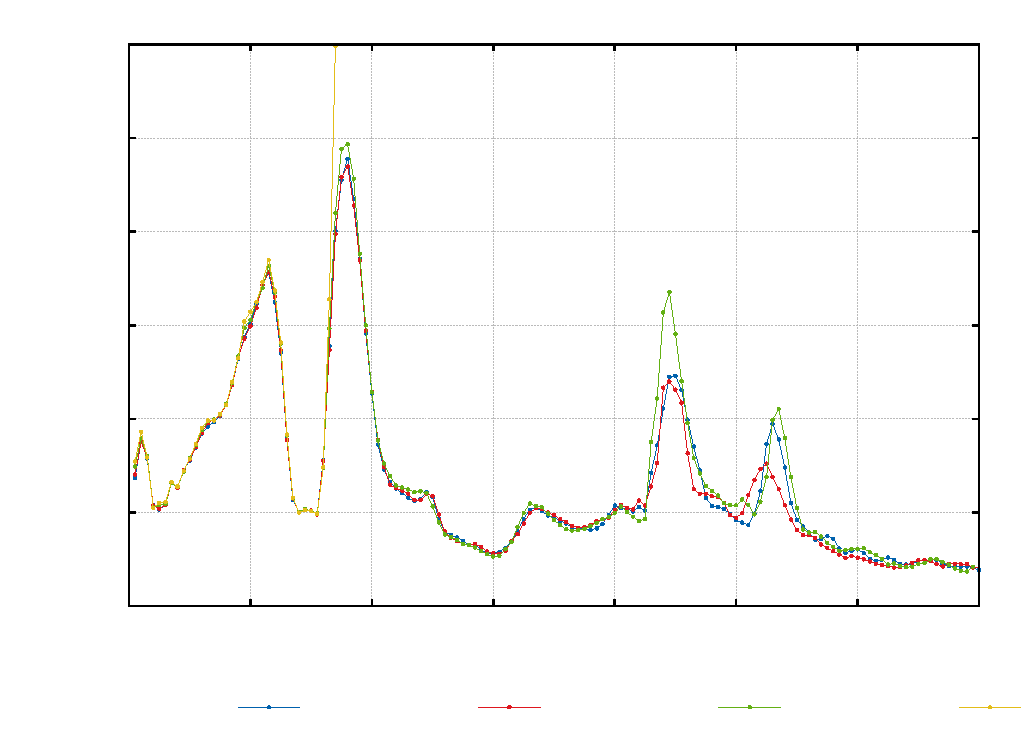
\includegraphics{et_dt}}%
    \gplfronttext
  \end{picture}%
\endgroup

\caption{Wykres energii kinetycznej cząstek od czasu $E_c(t)$ w zależności od kroku czasowego $\Delta t$}
\label{fig:plot_timestep}
\end{figure}

\par
Wykres \eqref{fig:plot_timestep} obrazuje po pierwsze stabilność symulacji ze względu na wielkość kroku czasowego, a po drugie podobieństwo przebiegu symulacji przy różnych wartościach kroku czasowego.
\par
Można zauważyć, że - gdy wielkość kroku czasowego nie jest za duża i nie powoduje eksplozji numerycznej - ma stosunkowo mały wpływ na zachowanie symulacji. Przebieg krzywych na wykresie (za wyjątkiem dwóch momentów) znacząco od siebie nie odbiega.

\begin{figure}[H]
% GNUPLOT: LaTeX picture with Postscript
\begingroup
  \makeatletter
  \providecommand\color[2][]{%
    \GenericError{(gnuplot) \space\space\space\@spaces}{%
      Package color not loaded in conjunction with
      terminal option `colourtext'%
    }{See the gnuplot documentation for explanation.%
    }{Either use 'blacktext' in gnuplot or load the package
      color.sty in LaTeX.}%
    \renewcommand\color[2][]{}%
  }%
  \providecommand\includegraphics[2][]{%
    \GenericError{(gnuplot) \space\space\space\@spaces}{%
      Package graphicx or graphics not loaded%
    }{See the gnuplot documentation for explanation.%
    }{The gnuplot epslatex terminal needs graphicx.sty or graphics.sty.}%
    \renewcommand\includegraphics[2][]{}%
  }%
  \providecommand\rotatebox[2]{#2}%
  \@ifundefined{ifGPcolor}{%
    \newif\ifGPcolor
    \GPcolortrue
  }{}%
  \@ifundefined{ifGPblacktext}{%
    \newif\ifGPblacktext
    \GPblacktextfalse
  }{}%
  % define a \g@addto@macro without @ in the name:
  \let\gplgaddtomacro\g@addto@macro
  % define empty templates for all commands taking text:
  \gdef\gplbacktext{}%
  \gdef\gplfronttext{}%
  \makeatother
  \ifGPblacktext
    % no textcolor at all
    \def\colorrgb#1{}%
    \def\colorgray#1{}%
  \else
    % gray or color?
    \ifGPcolor
      \def\colorrgb#1{\color[rgb]{#1}}%
      \def\colorgray#1{\color[gray]{#1}}%
      \expandafter\def\csname LTw\endcsname{\color{white}}%
      \expandafter\def\csname LTb\endcsname{\color{black}}%
      \expandafter\def\csname LTa\endcsname{\color{black}}%
      \expandafter\def\csname LT0\endcsname{\color[rgb]{1,0,0}}%
      \expandafter\def\csname LT1\endcsname{\color[rgb]{0,1,0}}%
      \expandafter\def\csname LT2\endcsname{\color[rgb]{0,0,1}}%
      \expandafter\def\csname LT3\endcsname{\color[rgb]{1,0,1}}%
      \expandafter\def\csname LT4\endcsname{\color[rgb]{0,1,1}}%
      \expandafter\def\csname LT5\endcsname{\color[rgb]{1,1,0}}%
      \expandafter\def\csname LT6\endcsname{\color[rgb]{0,0,0}}%
      \expandafter\def\csname LT7\endcsname{\color[rgb]{1,0.3,0}}%
      \expandafter\def\csname LT8\endcsname{\color[rgb]{0.5,0.5,0.5}}%
    \else
      % gray
      \def\colorrgb#1{\color{black}}%
      \def\colorgray#1{\color[gray]{#1}}%
      \expandafter\def\csname LTw\endcsname{\color{white}}%
      \expandafter\def\csname LTb\endcsname{\color{black}}%
      \expandafter\def\csname LTa\endcsname{\color{black}}%
      \expandafter\def\csname LT0\endcsname{\color{black}}%
      \expandafter\def\csname LT1\endcsname{\color{black}}%
      \expandafter\def\csname LT2\endcsname{\color{black}}%
      \expandafter\def\csname LT3\endcsname{\color{black}}%
      \expandafter\def\csname LT4\endcsname{\color{black}}%
      \expandafter\def\csname LT5\endcsname{\color{black}}%
      \expandafter\def\csname LT6\endcsname{\color{black}}%
      \expandafter\def\csname LT7\endcsname{\color{black}}%
      \expandafter\def\csname LT8\endcsname{\color{black}}%
    \fi
  \fi
  \setlength{\unitlength}{0.0500bp}%
  \begin{picture}(9636.00,6802.00)%
    \gplgaddtomacro\gplbacktext{%
      \csname LTb\endcsname%
      \put(946,1364){\makebox(0,0)[r]{\strut{} 0}}%
      \csname LTb\endcsname%
      \put(946,2103){\makebox(0,0)[r]{\strut{} 20}}%
      \csname LTb\endcsname%
      \put(946,2842){\makebox(0,0)[r]{\strut{} 40}}%
      \csname LTb\endcsname%
      \put(946,3581){\makebox(0,0)[r]{\strut{} 60}}%
      \csname LTb\endcsname%
      \put(946,4320){\makebox(0,0)[r]{\strut{} 80}}%
      \csname LTb\endcsname%
      \put(946,5059){\makebox(0,0)[r]{\strut{} 100}}%
      \csname LTb\endcsname%
      \put(946,5798){\makebox(0,0)[r]{\strut{} 120}}%
      \csname LTb\endcsname%
      \put(946,6537){\makebox(0,0)[r]{\strut{} 140}}%
      \csname LTb\endcsname%
      \put(1078,1144){\makebox(0,0){\strut{} 0}}%
      \csname LTb\endcsname%
      \put(2244,1144){\makebox(0,0){\strut{} 0.4}}%
      \csname LTb\endcsname%
      \put(3410,1144){\makebox(0,0){\strut{} 0.8}}%
      \csname LTb\endcsname%
      \put(4576,1144){\makebox(0,0){\strut{} 1.2}}%
      \csname LTb\endcsname%
      \put(5741,1144){\makebox(0,0){\strut{} 1.6}}%
      \csname LTb\endcsname%
      \put(6907,1144){\makebox(0,0){\strut{} 2}}%
      \csname LTb\endcsname%
      \put(8073,1144){\makebox(0,0){\strut{} 2.4}}%
      \csname LTb\endcsname%
      \put(9239,1144){\makebox(0,0){\strut{} 2.8}}%
      \csname LTb\endcsname%
      \put(176,3950){\rotatebox{-270}{\makebox(0,0){\strut{}$E_c(t)$}}}%
      \put(5158,814){\makebox(0,0){\strut{}$t$}}%
    }%
    \gplgaddtomacro\gplfronttext{%
      \csname LTb\endcsname%
      \put(3216,393){\makebox(0,0)[r]{\strut{}$s = 1000$}}%
      \csname LTb\endcsname%
      \put(3216,173){\makebox(0,0)[r]{\strut{}$s = 5000$}}%
      \csname LTb\endcsname%
      \put(5391,393){\makebox(0,0)[r]{\strut{}$s = 10000$}}%
      \csname LTb\endcsname%
      \put(5391,173){\makebox(0,0)[r]{\strut{}$s = 100000$}}%
      \csname LTb\endcsname%
      \put(7566,393){\makebox(0,0)[r]{\strut{}$s = 200000$}}%
    }%
    \gplbacktext
    \put(0,0){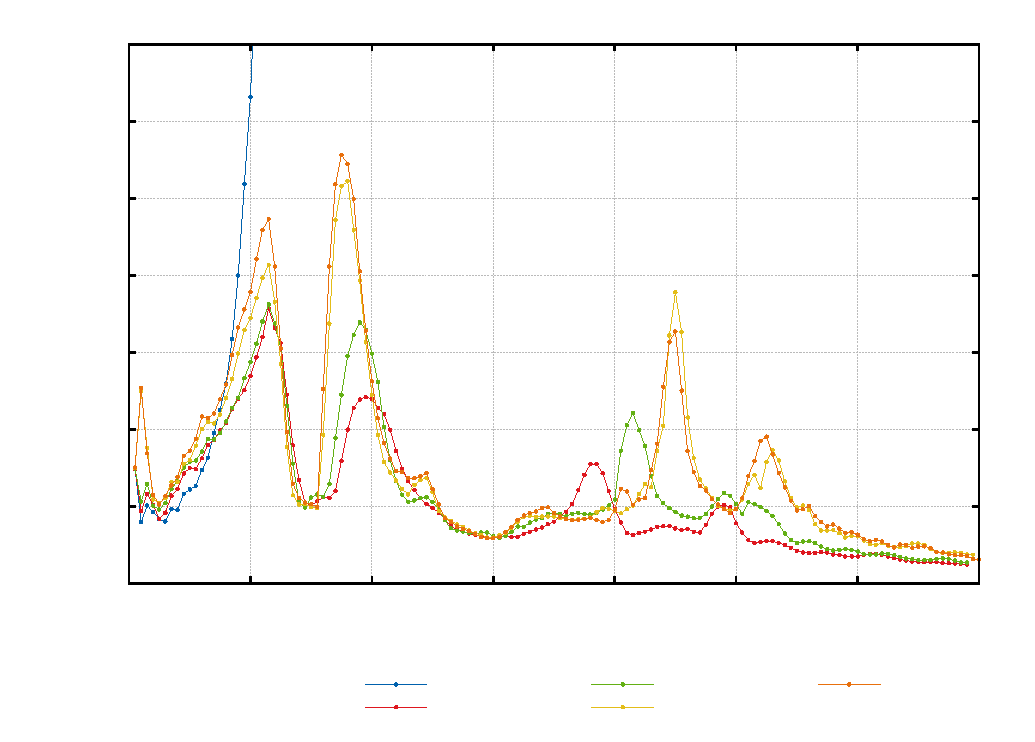
\includegraphics{et_stiff}}%
    \gplfronttext
  \end{picture}%
\endgroup

\caption{Wykres energii kinetycznej cząstek od czasu $E_c(t)$ w zależności od parametru sztywności ścianek $s$}
\label{fig:plot_stiff}
\end{figure}

\par
Wykres \eqref{fig:plot_stiff} przedstawia zachowanie się ścianek naczynia -- mniejsza wartość parametru $s$ oznacza większą `sprężystość' tych ścianek przez co duża część energii cząsteczek jest pochłaniana. Jednak gdy parametr $s$ zostanie ustalony na zbyt niską wartość, siła sprężystości jaką ścianki oddziałują na cząsteczki jest zbyt mała i następuje penetracja ścianek przez cząstki -- co widać na wykresie w momencie $t=0.4$ dla $s=1000$.
\par
W praktyce zmniejszenie parametru $s$ pozwala na delikatne poprawienie stabilności numerycznej. Powoduje jednak nienaturalnie wyglądające kolizje cząstek ze ścianami przez co domyślnie ten parametr został ustawiony na stosunkowo wysoką wartość.
\par